%%%%%%%%%%%%%%%%%%%%%%%%%%%%%%%%%%%%%%%%%
% Beamer Presentation
% LaTeX Template
% Version 1.0 (10/11/12)
%
% This template has been downloaded from:
% http://www.LaTeXTemplates.com
%
% License:
% CC BY-NC-SA 3.0 (http://creativecommons.org/licenses/by-nc-sa/3.0/)
%
%%%%%%%%%%%%%%%%%%%%%%%%%%%%%%%%%%%%%%%%%

%----------------------------------------------------------------------------------------
%	PACKAGES AND THEMES
%----------------------------------------------------------------------------------------

\documentclass{beamer}

\mode<presentation> {

% The Beamer class comes with a number of default slide themes
% which change the colors and layouts of slides. Below this is a list
% of all the themes, uncomment each in turn to see what they look like.

%\usetheme{default}
%\usetheme{AnnArbor}
%\usetheme{Antibes}
%\usetheme{Bergen}
%\usetheme{Berkeley}
%\usetheme{Berlin}
%\usetheme{Boadilla}
%\usetheme{CambridgeUS}
%\usetheme{Copenhagen}
%\usetheme{Darmstadt}
%\usetheme{Dresden}
%\usetheme{Frankfurt}
%\usetheme{Goettingen}
%\usetheme{Hannover}
%\usetheme{Ilmenau}
%\usetheme{JuanLesPins}
%\usetheme{Luebeck}
%\usetheme{Madrid}
%\usetheme{Malmoe}
%\usetheme{Marburg}
%\usetheme{Montpellier}
%\usetheme{PaloAlto}
\usetheme{Pittsburgh}
%\usetheme{Rochester}
%\usetheme{Singapore}
%\usetheme{Szeged}
%\usetheme{Warsaw}

% As well as themes, the Beamer class has a number of color themes
% for any slide theme. Uncomment each of these in turn to see how it
% changes the colors of your current slide theme.

%\usecolortheme{albatross}
\usecolortheme{beaver}
%\usecolortheme{beetle}
%\usecolortheme{crane}
%\usecolortheme{dolphin}
%\usecolortheme{dove}
%\usecolortheme{fly}
%\usecolortheme{lily}
%\usecolortheme{orchid}
%\usecolortheme{rose}
%\usecolortheme{seagull}
%\usecolortheme{seahorse}
%\usecolortheme{whale}
%\usecolortheme{wolverine}

%\setbeamertemplate{footline} % To remove the footer line in all slides uncomment this line
%\setbeamertemplate{footline}[page number] % To replace the footer line in all slides with a simple slide count uncomment this line

%\setbeamertemplate{navigation symbols}{} % To remove the navigation symbols from the bottom of all slides uncomment this line
}
\usepackage{graphicx} % Allows including images
\usepackage{booktabs} % Allows the use of \toprule, \midrule and \bottomrule in tables

\usepackage{fontspec}
\setsansfont{Calibri}[
    Path=Font/,
    Scale=0.9,
    Extension = .ttf,
    UprightFont=*-Regular,
    BoldFont=*-Bold,
    ItalicFont=*-Italic,
    BoldItalicFont=*-BoldItalic
    ]
\usepackage{unicode-math}
\setmathfont{Libertinus Math}% 使用默认的数学字体或你偏好的数学字体 Latin Modern Math/Libertinus Math
% \setmathfont[version=bold]{Latin Modern Math}

\usepackage{ragged2e}
\justifying\let\raggedright\justifying %两端对齐
%----------------------------------------------------------------------------------------
%	TITLE PAGE
%----------------------------------------------------------------------------------------

\title[Asset Pricing]{\textbf{Asset Pricing}} % The short title appears at the bottom of every slide, the full title is only on the title page

\subtitle{5. Production-Based Asset Pricing}

\author[Cheng Hang]{Cheng Hang} % Your name
\institute[DUFE] % Your institution as it will appear on the bottom of every slide, may be shorthand to save space
{School of Fintech \\
Dongbei University of Finance \& Economics \\ % Your institution for the title page
\medskip
\textbf{chenghangch@qq.com}% Your email address
}
\date{\today} % Date, can be changed to a custom date

	\AtBeginSection[]
{
	\begin{frame}{Content}
		\tableofcontents[sectionstyle=show/shaded,subsectionstyle=show/shaded/hide] %这几个参数我也不知道该如何准确地解释，反正它们最终的效果是突出显示当前章节，而其它章节都进行了淡化处理
		\addtocounter{framenumber}{-1}  %目录页不计算页码
	\end{frame}
}

%----------------------------------------------------------------------------------------
%	Begin
%----------------------------------------------------------------------------------------

\begin{document}

\begin{frame}
\titlepage % Print the title page as the first slide
\end{frame}

%\begin{frame}
%\frametitle{Overview} % Table of contents slide, comment this block out to remove it
%\tableofcontents % Throughout your presentation, if you choose to use \section{} and \subsection{} commands, these will automatically be printed on this slide as an overview of your presentation
%\end{frame}

%--------------------------------------
%	PRESENTATION SLIDES
%--------------------------------------


\begin{frame}
	\begin{figure}
		\centering
		
\includegraphics[width=1\linewidth]{Files/qfactor.jpg}
	\end{figure}
\end{frame}


\begin{frame}{From Demand-Side to Supply-Side: The Evolution}
    \textbf{Traditional Demand-Side Asset Pricing:}
    \begin{itemize}
        \item \textbf{CAPM (Sharpe, 1964; Lintner, 1965):} Investor optimization $\rightarrow$ Expected returns
        \item \textbf{Consumption CAPM (\href{https://www.jstor.org/stable/1913837}{\textcolor{blue}{Lucas, 1978}}; \href{https://www.sciencedirect.com/science/article/pii/0304405X79900163}{\textcolor{blue}{Breeden, 1979}}):} Consumption risk
        \item \textbf{Fama-French (1993):} Empirical factors (SMB, HML)
    \end{itemize}
    
    
    \textbf{Problems with Demand-Side Approach:}
    \begin{itemize}
        \item \textbf{Factors often lack clear theoretical foundation}
        \item ``Joint hypothesis problem" (Fama, 1991): Model or efficiency?
        \item Disconnect between corporate finance and asset pricing
    \end{itemize}
    
    
    \textbf{The Production-Based Alternative:}
    \begin{itemize}
        \item Start from \textit{firms' investment decisions}, not investors' portfolios
        \item Use NPV rule: Firms invest until marginal $q = 1$
        \item Link corporate finance fundamentals to asset returns
        \item \textcolor{blue}{\href{https://doi.org/10.1111/j.1540-6261.1991.tb03750.x }{Cochrane (1991)}}, \textcolor{blue}{\href{https://doi.org/10.1086/649760}{Liu, Whited, and Zhang (2009)}}
    \end{itemize}
\end{frame}

\begin{frame}{Core Intuition: Why Production Matters for Returns}
    \textbf{The Fundamental Equality:}
    \begin{equation*}
        \underbrace{\text{Financial Return}}_{\text{Stock market}} = \underbrace{\text{Investment Return}}_{\text{Real economy}}
    \end{equation*}
    
    
    \textbf{Economic Intuition:}
    \begin{itemize}
        \item In equilibrium, return on \textit{financial claims} to firm = return on \textit{physical investment}
        \item If financial returns $>$ investment returns $\rightarrow$ Arbitrage: Invest more
        \item If financial returns $<$ investment returns $\rightarrow$ Disinvest, return cash
        \item Firms' optimization pins down the cross-section of expected returns
    \end{itemize}
    
    
    \textbf{Key Insight:}
    \begin{itemize}
        \item Firms with different investment and profitability characteristics face different investment returns
        \item These differences in investment returns must equal differences in financial returns
        \item $\Rightarrow$ Investment and profitability predict stock returns
    \end{itemize}
\end{frame}

\begin{frame}{The Production-Based Framework}
    \textbf{Key Components:}
    \begin{enumerate}
        \item \textbf{Technology:} Cobb-Douglas production function
        \begin{equation*}
            X_t = Z_t K_t^\alpha L_t^{1-\alpha}
        \end{equation*}
        
        \item \textbf{Adjustment Costs:} Convex costs of changing capital stock
        \begin{equation*}
            \Phi_t = \phi\left(\frac{I_t}{K_t}\right) K_t, \quad \phi' > 0, \quad \phi'' \geq 0
        \end{equation*}
        
        \item \textbf{Optimization:} Firms maximize value subject to technology and costs
        \begin{equation*}
            V_t = \max \mathrm{E}_t \sum_{s=0}^{\infty} M_{t,t+s} D_{t+s}
        \end{equation*}
        
        \item \textbf{Key Result:} Investment and profitability determine returns
    \end{enumerate}
    
    \vspace{0.2cm}
    \textbf{Following:} \textcolor{blue}{\href{https://doi.org/10.1146/annurev-financial-110311-101731}{Kogan and Papanikolaou (2012)}} exposition
\end{frame}

\section{Building Blocks: Technology and Optimization}

\begin{frame}{Step 1: Production Technology}
    \textbf{Cobb-Douglas Production Function:}
    \begin{equation}\label{equ:production}
        X_t = Z_t K_t^\alpha L_t^{1-\alpha}
    \end{equation}
    where:
    \begin{itemize}
        \item $X_t$: Output (goods produced)
        \item $Z_t$: Total factor productivity (TFP) shock
        \item $K_t$: Capital stock (machines, equipment, buildings)
        \item $L_t$: Labor input (workers)
        \item $\alpha \in (0,1)$: Capital share of output
    \end{itemize}
    
    
    \textbf{Properties:}
    \begin{itemize}
        \item \textbf{Constant returns to scale:} $X_t(\lambda K, \lambda L) = \lambda X_t(K,L)$
        \item \textbf{Diminishing marginal products:} $\frac{\partial^2 X}{\partial K^2} < 0$, $\frac{\partial^2 X}{\partial L^2} < 0$
        \item \textbf{Capital share:} In equilibrium, $\alpha = \frac{K \cdot MPK}{X}$ (capital income / output)
    \end{itemize}
\end{frame}

\begin{frame}{Step 2: Optimal Labor Choice}
    \textbf{Firm's Labor Decision:}
    \begin{itemize}
        \item Take capital $K_t$ and wage $\omega_t$ as given
        \item Choose labor $L_t$ to maximize short-run profits
        \item First-order condition: Marginal product = Wage
    \end{itemize}
    
    \vspace{0.2cm}
    \textbf{Derivation:}
    \begin{equation*}
        \max_{L_t} \left\{ X_t - \omega_t L_t \right\} \quad \Rightarrow \quad \frac{\partial X_t}{\partial L_t} = \omega_t
    \end{equation*}
    
    \begin{equation*}
        (1-\alpha) Z_t K_t^\alpha L_t^{-\alpha} = \omega_t
    \end{equation*}
    
    \textbf{Optimal Labor Demand:}
    \begin{equation}\label{equ:optimal labor supply}
        L_t^* = \left(\frac{(1-\alpha)Z_t}{\omega_t}\right)^{1/\alpha} K_t
    \end{equation}
    
    \vspace{0.2cm}
    \textbf{Economic Interpretation:}
    \begin{itemize}
        \item Labor demand increases in productivity $Z_t$ and capital $K_t$
        \item Labor demand decreases in wage $\omega_t$
        \item Elasticity of labor demand: $1/\alpha$ (typically $\alpha \approx 1/3$, so elasticity $\approx 3$)
    \end{itemize}
\end{frame}

\begin{frame}{Step 3: Output Given Optimal Labor}
    \textbf{Substituting $L_t^*$ into Production Function:}
    \begin{equation*}
        \begin{aligned}
            Y_t &= Z_t K_t^\alpha \left(L_t^*\right)^{1-\alpha} \\
            &= Z_t K_t^\alpha \left[\left(\frac{(1-\alpha)Z_t}{\omega_t}\right)^{1/\alpha} K_t\right]^{1-\alpha} \\
            &= Z_t K_t^\alpha \cdot \left(\frac{(1-\alpha)Z_t}{\omega_t}\right)^{(1-\alpha)/\alpha} \cdot K_t^{1-\alpha} \\
            &= Z_t^{1/\alpha} \left(\frac{1-\alpha}{\omega_t}\right)^{(1-\alpha)/\alpha} K_t
        \end{aligned}
    \end{equation*}
    
    \textbf{Key Insight: Output-Capital Ratio}
    \begin{equation*}
        \frac{Y_t}{K_t} = Z_t^{1/\alpha} \left(\frac{1-\alpha}{\omega_t}\right)^{(1-\alpha)/\alpha}
    \end{equation*}
    
    \begin{itemize}
        \item Output per unit of capital depends on productivity $Z_t$ and wage $\omega_t$
        \item Higher productivity $\rightarrow$ higher output-capital ratio
        \item Higher wages $\rightarrow$ lower output-capital ratio (labor is expensive)
        \item This ratio is crucial for measuring profitability
    \end{itemize}
\end{frame}

\begin{frame}{Step 4: Gross Profits}
    \textbf{Profits After Paying Labor:}
    \begin{equation}\label{equ: gross profit}
        \begin{aligned}
            \Pi_t &= Y_t - \omega_t L_t^* \\
            &= Y_t - \omega_t \left(\frac{(1-\alpha)Z_t}{\omega_t}\right)^{1/\alpha} K_t \\
            &= Y_t - (1-\alpha)^{1/\alpha} Z_t^{1/\alpha} \omega_t^{1-1/\alpha} K_t
        \end{aligned}
    \end{equation}
    
    \textbf{Simplification Using Output Expression:}
    \begin{equation*}
        \begin{aligned}
            \Pi_t &= Y_t - (1-\alpha) \cdot \underbrace{Z_t^{1/\alpha} \left(\frac{1-\alpha}{\omega_t}\right)^{(1-\alpha)/\alpha} K_t}_{= Y_t} \\
            &= Y_t - (1-\alpha) Y_t \\
            &= \alpha Y_t
        \end{aligned}
    \end{equation*}
    
    \vspace{0.2cm}
    \textbf{Economic Interpretation:}
    \begin{itemize}
        \item Capital share $\alpha$ is the fraction of output paid to capital owners
        \item Labor share $(1-\alpha)$ is the fraction paid to workers
        \item Standard result in Cobb-Douglas models
        \item Empirically, $\alpha \approx 1/3$ in US data
    \end{itemize}
\end{frame}

\section{Investment Decision with Adjustment Costs}

\begin{frame}{Why Adjustment Costs Matter}
    \textbf{Without Adjustment Costs:}
    \begin{itemize}
        \item Firms adjust capital instantaneously to optimal level
        \item Investment is infinitely elastic to Tobin's $q$
        \item Contradicts observed sluggish investment behavior
    \end{itemize}
    
    
    \textbf{With Adjustment Costs (Lucas, 1967; Hayashi, 1982):}
    \begin{itemize}
        \item Costly to install new capital or reduce capital stock
        \item Includes:
        \begin{itemize}
            \item Installation costs (training workers on new equipment)
            \item Disruption of production during installation
            \item Search costs for finding buyers/sellers of capital
            \item Organizational restructuring costs
        \end{itemize}
        \item Creates inertia in investment decisions
        \item Makes investment forward-looking: depends on future profitability
    \end{itemize}
\end{frame}

\begin{frame}{Capital Accumulation and Investment Costs}
    \textbf{Law of Motion for Capital:}
    \begin{equation}\label{equ:capital accumulation}
        K_{t+1} = I_t + (1-\delta)K_t
    \end{equation}
    where $\delta \in (0,1)$ is the depreciation rate
    
    
    \textbf{Total Cost of Investment:}
    \begin{equation}\label{equ:investment cost}
        \Phi_t = \phi\left(\frac{I_t}{K_t}\right) K_t
    \end{equation}
    
    \textbf{Properties of $\phi(\cdot)$ Function:}
    \begin{enumerate}
        \item $\phi' > 0$ when $I > 0$: Marginal cost increases with investment rate
        \item $\phi'' \geq 0$: Convex (accelerating costs)
        \item $\phi(0) = 0$: No cost if no investment
        \item Homogeneity: Only depends on investment rate $I_t/K_t$, not levels
    \end{enumerate}
    
    \vspace{0.2cm}
    \textbf{Without adjustment costs:} $\phi(I_t/K_t) = I_t/K_t$, so $\Phi_t = I_t$ (just pay for capital)
\end{frame}

\begin{frame}{Dividends and Firm Value}
    \textbf{Dividends (Cash Flow to Shareholders):}
    \begin{equation}\label{equ:dividend}
        D_t = \Pi_t - \Phi_t = \alpha Y_t - \phi\left(\frac{I_t}{K_t}\right) K_t
    \end{equation}
    
    \begin{itemize}
        \item Profits from operations $\Pi_t = \alpha Y_t$
        \item Minus investment costs $\Phi_t$
        \item What's left can be paid out
    \end{itemize}
    
    
    \textbf{Firm Value (Present Value of Dividends):}
    \begin{equation}\label{equ:firm value}
        V_t = \mathrm{E}_t \sum_{s=0}^{\infty} M_{t,t+s} D_{t+s}
    \end{equation}
    
    where $M_{t,t+s}$ is the stochastic discount factor from $t$ to $t+s$
    
    
    \textbf{Interpretation:}
    \begin{itemize}
        \item Firm is worth the discounted stream of cash flows
        \item Managers choose investment $I_t$ to maximize $V_t$
        \item Key: Current investment affects \textit{all future} cash flows via capital accumulation
    \end{itemize}
\end{frame}

\section{The Firm's Optimization Problem}

\begin{frame}{Dynamic Programming Formulation}
    \textbf{Bellman Equation:}
    \begin{equation}\label{equ:bellman}
        V_t = \max_{I_t} \left\{ D_t + \mathrm{E}_t\left[M_{t+1} V_{t+1}\right] \right\}
    \end{equation}
    
    \textbf{Interpretation:}
    \begin{itemize}
        \item Today's value = Today's dividend + Discounted expected future value
        \item Choice variable: Investment $I_t$
        \item Trade-off:
        \begin{itemize}
            \item Higher $I_t$ $\rightarrow$ Lower $D_t$ today (costs money)
            \item But higher $K_{t+1}$ $\rightarrow$ Higher $V_{t+1}$ tomorrow (more production)
        \end{itemize}
    \end{itemize}
    
    
    \textbf{First-Order Condition:}
    \begin{equation}\label{equ:foc}
        \frac{\partial D_t}{\partial I_t} + \mathrm{E}_t\left[M_{t+1} \frac{\partial V_{t+1}}{\partial I_t}\right] = 0
    \end{equation}
    
    Using $\frac{\partial D_t}{\partial I_t} = -\phi'\left(\frac{I_t}{K_t}\right)$ and $\frac{\partial V_{t+1}}{\partial I_t} = \frac{\partial V_{t+1}}{\partial K_{t+1}}$:
    \begin{equation}\label{equ:marginal}
        \phi'\left(\frac{I_t}{K_t}\right) = \mathrm{E}_t\left[M_{t+1} \frac{\partial V_{t+1}}{\partial K_{t+1}}\right]
    \end{equation}
\end{frame}

\begin{frame}[allowframebreaks]{Interpreting the First-Order Condition}
    \begin{equation*}
        \underbrace{\phi'\left(\frac{I_t}{K_t}\right)}_{\text{Marginal cost of investing}} = \underbrace{\mathrm{E}_t\left[M_{t+1} \frac{\partial V_{t+1}}{\partial K_{t+1}}\right]}_{\text{Expected discounted marginal benefit}}
    \end{equation*}
    
    
    \textbf{Left-Hand Side (Marginal Cost):}
    \begin{itemize}
        \item Cost of investing one more unit today
        \item Includes purchase price + adjustment costs
        \item Reduces current dividends
    \end{itemize}
    
    
    \textbf{Right-Hand Side (Marginal Benefit):}
    \begin{itemize}
        \item Value of having one more unit of capital tomorrow
        \item Discounted by SDF $M_{t+1}$ (adjust for risk and time preference)
        \item Increases future production and profits
    \end{itemize}
    
    
    \textbf{Equilibrium:}
    \begin{itemize}
        \item Invest until marginal cost = expected marginal benefit
        \item If $\phi' < \mathrm{E}[M V']$: Invest more (benefit exceeds cost)
        \item If $\phi' > \mathrm{E}[M V']$: Invest less (cost exceeds benefit)
    \end{itemize}
\end{frame}

\begin{frame}{The Envelope Theorem}
    \textbf{What is the Marginal Value of Capital?}
    
    Differentiate Bellman equation (\ref{equ:bellman}) with respect to $K_t$ and advance one period:
    \begin{equation}\label{equ:envelope}
        \frac{\partial V_{t+1}}{\partial K_{t+1}} = \frac{\partial D_{t+1}}{\partial K_{t+1}} + \mathrm{E}_{t+1}\left[M_{t+2} \frac{\partial V_{t+2}}{\partial K_{t+1}}\right]
    \end{equation}
    
    \textbf{Step 1: Compute $\frac{\partial D_{t+1}}{\partial K_{t+1}}$}
    \begin{equation*}
        \begin{aligned}
            \frac{\partial D_{t+1}}{\partial K_{t+1}} &= \frac{\partial}{\partial K_{t+1}}\left[\alpha Y_{t+1} - \phi\left(\frac{I_{t+1}}{K_{t+1}}\right) K_{t+1}\right] \\
            &= \alpha \frac{\partial Y_{t+1}}{\partial K_{t+1}} - \frac{\partial}{\partial K_{t+1}}\left[\phi\left(\frac{I_{t+1}}{K_{t+1}}\right) K_{t+1}\right]
        \end{aligned}
    \end{equation*}
    
    The investment cost term:
    \begin{equation*}
        \frac{\partial \Phi_{t+1}}{\partial K_{t+1}} = \phi\left(\frac{I_{t+1}}{K_{t+1}}\right) - \phi'\left(\frac{I_{t+1}}{K_{t+1}}\right) \frac{I_{t+1}}{K_{t+1}}
    \end{equation*}
\end{frame}

\begin{frame}{The Envelope Theorem (cont.)}
    \textbf{Step 2: Use Chain Rule on Future Value Term}
    \begin{equation*}
        \frac{\partial V_{t+2}}{\partial K_{t+1}} = \frac{\partial V_{t+2}}{\partial K_{t+2}} \cdot \frac{\partial K_{t+2}}{\partial K_{t+1}} = \frac{\partial V_{t+2}}{\partial K_{t+2}} (1-\delta)
    \end{equation*}
    
    because $K_{t+2} = I_{t+1} + (1-\delta)K_{t+1}$ (only undepreciated capital matters)
    
    
    \textbf{Step 3: Apply FOC (\ref{equ:marginal}) One Period Forward}
    \begin{equation*}
        \mathrm{E}_{t+1}\left[M_{t+2} \frac{\partial V_{t+2}}{\partial K_{t+2}}\right] = \phi'\left(\frac{I_{t+1}}{K_{t+1}}\right)
    \end{equation*}
    
    
    \textbf{Final Result (Envelope Theorem):}
    \begin{equation}\label{equ:envelope theorem}
        \boxed{
        \frac{\partial V_{t+1}}{\partial K_{t+1}} = \alpha \frac{\partial Y_{t+1}}{\partial K_{t+1}} - \frac{\partial \Phi_{t+1}}{\partial K_{t+1}} + (1-\delta) \phi'\left(\frac{I_{t+1}}{K_{t+1}}\right)
        }
    \end{equation}
\end{frame}

\begin{frame}{Economic Interpretation of the Envelope Theorem}
    \begin{equation*}
        \frac{\partial V_{t+1}}{\partial K_{t+1}} = \underbrace{\alpha \frac{\partial Y_{t+1}}{\partial K_{t+1}}}_{\text{(1) Profit contribution}} - \underbrace{\frac{\partial \Phi_{t+1}}{\partial K_{t+1}}}_{\text{(2) Cost effect}} + \underbrace{(1-\delta) \phi'\left(\frac{I_{t+1}}{K_{t+1}}\right)}_{\text{(3) Scrap value}}
    \end{equation*}
    
    
    \textbf{Three Components:}
    \begin{enumerate}
        \item \textbf{Marginal Profit:} Extra output $\times$ profit share $\alpha$
        \begin{itemize}
            \item More capital $\rightarrow$ more production $\rightarrow$ more profits
        \end{itemize}
        
        \item \textbf{Cost Reduction:} Lower average adjustment costs
        \begin{itemize}
            \item Bigger capital base $\rightarrow$ same investment is smaller fraction
            \item Recall $\Phi = \phi(I/K) \cdot K$, so $\partial \Phi/\partial K < 0$ if $I > 0$
        \end{itemize}
        
        \item \textbf{Continuation Value:} Undepreciated capital carries forward
        \begin{itemize}
            \item Fraction $(1-\delta)$ survives to next period
            \item Worth its marginal cost of installation $\phi'$
        \end{itemize}
    \end{enumerate}
    
    \vspace{0.2cm}
    \textit{The marginal value of capital equals the sum of its immediate profit contribution and its continuation value}
\end{frame}

\section{Constant Returns to Scale: Tobin's Q}

\begin{frame}{Hayashi's (1982) Key Result}
    \textbf{Assumption: Constant Returns to Scale (CRS)}
    \begin{itemize}
        \item Production: $X_t = Z_t K_t^\alpha L_t^{1-\alpha}$ exhibits CRS
        \item Adjustment costs: $\Phi_t = \phi(I_t/K_t) K_t$ exhibits CRS in $(I_t, K_t)$
    \end{itemize}
    
    
    \textbf{Hayashi's Theorem:}
    
    Under CRS, marginal $q$ equals average $q$:
    \begin{equation}\label{equ:hayashi}
        \boxed{
        \frac{\partial V_t}{\partial K_t} = \frac{V_t}{K_t}
        }
    \end{equation}
    
    
    \textbf{Intuition:}
    \begin{itemize}
        \item CRS $\rightarrow$ doubling all inputs doubles output and value
        \item Marginal and average products are equal
        \item Value of firm = Marginal value of capital $\times$ Quantity of capital
        \item Key simplification: Don't need to estimate marginal $q$, just use $V/K$
    \end{itemize}
\end{frame}

\begin{frame}{Deriving Tobin's Q Equation}
    \textbf{Start with FOC (\ref{equ:marginal}):}
    \begin{equation*}
        \phi'\left(\frac{I_t}{K_t}\right) = \mathrm{E}_t\left[M_{t+1} \frac{\partial V_{t+1}}{\partial K_{t+1}}\right]
    \end{equation*}
    
    \textbf{Apply Hayashi result (\ref{equ:hayashi}):}
    \begin{equation*}
        \phi'\left(\frac{I_t}{K_t}\right) = \mathrm{E}_t\left[M_{t+1} \frac{V_{t+1}}{K_{t+1}}\right]
    \end{equation*}
    
    \textbf{Use Bellman equation: $V_t = D_t + \mathrm{E}_t[M_{t+1} V_{t+1}]$}
    
    Since $K_{t+1}$ is known at time $t$:
    \begin{equation*}
        \phi'\left(\frac{I_t}{K_t}\right) = \frac{\mathrm{E}_t[M_{t+1} V_{t+1}]}{K_{t+1}} = \frac{V_t - D_t}{K_{t+1}}
    \end{equation*}
    
    \textbf{Final Form (Tobin's Q):}
    \begin{equation}\label{equ:tobins q}
        \boxed{
        \phi'\left(\frac{I_t}{K_t}\right) = \frac{V_t - D_t}{K_{t+1}} = \frac{D_t}{K_{t+1}} \cdot \frac{V_t - D_t}{D_t}
        }
    \end{equation}
\end{frame}

\begin{frame}[allowframebreaks]{Unpacking Tobin's Q}
    \begin{equation*}
        \phi'\left(\frac{I_t}{K_t}\right) = \underbrace{\frac{D_t}{K_{t+1}}}_{\text{Current profitability}} \times \underbrace{\frac{V_t - D_t}{D_t}}_{\text{Price-dividend ratio}}
    \end{equation*}
    
    
    \textbf{Left Side: Marginal Cost of Investment}
    \begin{itemize}
        \item How expensive is it to invest today?
        \item Higher investment rate $\rightarrow$ higher marginal cost (convexity)
    \end{itemize}
    
    
    \textbf{Right Side, First Term: Current Profitability}
    \begin{itemize}
        \item $D_t/K_{t+1}$: Dividend per unit of tomorrow's capital
        \item Measures how profitable capital is \textit{right now}
        \item High if firm is generating lots of cash flow
    \end{itemize}
    
    
    \textbf{Right Side, Second Term: Growth Opportunities}
    \begin{itemize}
        \item $(V_t - D_t)/D_t$: Market value minus current dividend, per dollar of dividend
        \item High if market expects strong future dividend growth
        \item Related to $q$: ratio of market value to replacement cost
    \end{itemize}
\end{frame}

\begin{frame}{Tobin's Q: Economic Content}
    \textbf{High Investment Firms ($I_t/K_t$ large):}
    \begin{itemize}
        \item Left side: $\phi'$ is high (expensive to invest so much)
        \item Right side must also be high, so:
        \begin{itemize}
            \item \textbf{Either} high current profitability $D_t/K_{t+1}$
            \item \textbf{Or} high valuation $(V_t - D_t)/D_t$ (strong growth prospects)
            \item \textbf{Or both}
        \end{itemize}
    \end{itemize}
    
    
    \textbf{Low Investment Firms ($I_t/K_t$ small):}
    \begin{itemize}
        \item Left side: $\phi'$ is low (cheap marginal unit)
        \item Right side must also be low:
        \begin{itemize}
            \item Low current profitability
            \item Or poor growth prospects
            \item Or both
        \end{itemize}
    \end{itemize}
    
    
    \textbf{Key Insight:}
    \begin{itemize}
        \item Investment decisions reveal information about profitability and growth
        \item Can infer expected returns from observable investment behavior
    \end{itemize}
\end{frame}

\section{The Investment-Return Relation}

\begin{frame}{From Q-Theory to Expected Returns}
    \textbf{Campbell-Shiller Log-Linearization:}
    
    Take logs and apply Campbell-Shiller approximation to $V_t - D_t = V_t(1 - D_t/V_t)$:
    \begin{equation}\label{equ:campbell shiller}
        \log\left(\phi'\left(\frac{I_t}{K_t}\right)\right) \approx (d_t - k_{t+1}) + \mathrm{E}_t \sum_{j=0}^{\infty} \rho^j \Delta d_{t+1+j} - \mathrm{E}_t \sum_{j=0}^{\infty} \rho^j r_{t+1+j}
    \end{equation}
    
    where:
    \begin{itemize}
        \item $d_t = \log D_t$, $k_t = \log K_t$, $r_t$ is log return
        \item $\rho = 1 - \exp(\overline{d - v}) < 1$ is linearization constant
    \end{itemize}
    
    
    \textbf{Economic Interpretation:}
    \begin{equation*}
        \underbrace{\text{Invest more}}_{\phi' \uparrow} \Leftrightarrow \begin{cases}
            \text{High current profitability} & (d_t - k_{t+1}) \uparrow \\
            \text{Rapid dividend growth} & \sum \rho^j \Delta d_{t+1+j} \uparrow \\
            \text{OR low future returns} & \sum \rho^j r_{t+1+j} \downarrow
        \end{cases}
    \end{equation*}
\end{frame}

\begin{frame}{The Core Prediction: Investment and Returns}
    \textbf{Rearranging (\ref{equ:campbell shiller}):}
    \begin{equation*}
        \mathrm{E}_t \sum_{j=0}^{\infty} \rho^j r_{t+1+j} \approx (d_t - k_{t+1}) + \mathrm{E}_t \sum_{j=0}^{\infty} \rho^j \Delta d_{t+1+j} - \log\left(\phi'\left(\frac{I_t}{K_t}\right)\right)
    \end{equation*}
    
    \textbf{Holding profitability constant:}
    \begin{equation*}
        \frac{\partial \mathrm{E}_t[\sum r_{t+1+j}]}{\partial (I_t/K_t)} < 0
    \end{equation*}
    
    
    \textbf{Key Predictions:}
    \begin{enumerate}
        \item \textbf{Investment effect:} High investment $\rightarrow$ Low future returns
        \begin{itemize}
            \item Firms invest a lot when discount rates (required returns) are low
            \item Investing today reduces marginal productivity of capital tomorrow
        \end{itemize}
        
        \item \textbf{Profitability effect:} High profitability $\rightarrow$ High future returns
        \begin{itemize}
            \item Controlling for investment, profitable firms must offer higher returns
            \item Compensates for risk or reflects temporary mispricing
        \end{itemize}
    \end{enumerate}
\end{frame}

\begin{frame}{Intuition: Why Investment Predicts Returns}
    \textbf{Scenario 1: High Investment Firms}
    \begin{itemize}
        \item Currently investing heavily: $I_t/K_t$ is large
        \item Why? \textbf{Either:}
        \begin{itemize}
            \item Current profitability is high, OR
            \item Expected future profitability is high, OR
            \item Required returns (discount rates) are low
        \end{itemize}
        \item If we control for current and future profitability...
        \item Then high investment must mean low required returns
        \item $\Rightarrow$ Low future stock returns
    \end{itemize}
    
    
    \textbf{Scenario 2: Low Investment Firms}
    \begin{itemize}
        \item Currently investing little: $I_t/K_t$ is small
        \item Could be:
        \begin{itemize}
            \item Profitability is low, OR
            \item Required returns are high (capital is expensive)
        \end{itemize}
        \item Controlling for profitability...
        \item Low investment signals high required returns
        \item $\Rightarrow$ High future stock returns
    \end{itemize}
\end{frame}

\begin{frame}{Intuition: Why Profitability Predicts Returns}
    \textbf{Scenario 1: High Profitability, Low Investment}
    \begin{itemize}
        \item Firm is very profitable: $D_t/K_t$ is large
        \item But investing little: $I_t/K_t$ is small
        \item From Q-theory: $\phi'(I/K) = (D/K) \times (V-D)/D$
        \item Left side is low (low investment), first term on right is high
        \item So $(V-D)/D$ must be low $\rightarrow$ Market values firm cheaply
        \item $\Rightarrow$ High future returns (mean reversion or risk premium)
    \end{itemize}
    
    
    \textbf{Scenario 2: Low Profitability, High Investment}
    \begin{itemize}
        \item Firm has low current profits: $D_t/K_t$ is small
        \item But investing heavily: $I_t/K_t$ is large
        \item Left side is high, first term on right is low
        \item So $(V-D)/D$ must be high $\rightarrow$ Market values firm richly
        \item Expects future improvements, so current returns are low
        \item $\Rightarrow$ Low future returns
    \end{itemize}
    
    \vspace{0.2cm}
    \textbf{Key:} Investment and profitability together pin down expected returns
\end{frame}

\section{Liu, Whited, and Zhang (2009): Making It Empirical}

\begin{frame}{Specifying the Adjustment Cost Function}
    \textbf{Problem:} Q-theory gives general relationship, but need specific form for empirics
    
    \vspace{0.2cm}
    \textbf{Liu, Whited, and Zhang (2009) Specification:}
    \begin{equation}\label{equ:lwz cost}
        \phi\left(\frac{I_t}{K_t}\right) = \frac{I_t}{K_t} + \frac{a}{2}\left(\frac{I_t}{K_t}\right)^2
    \end{equation}
    
    where $a > 0$ is the adjustment cost parameter
    
    
    \textbf{Properties:}
    \begin{itemize}
        \item \textbf{Purchase cost:} $I_t/K_t$ (just buying the capital)
        \item \textbf{Quadratic adjustment cost:} $\frac{a}{2}(I_t/K_t)^2$ (installation, disruption)
        \item \textbf{Marginal cost:}
        \begin{equation}\label{equ:marginal cost}
            \phi'\left(\frac{I_t}{K_t}\right) = 1 + a\left(\frac{I_t}{K_t}\right)
        \end{equation}
        \item Linear in investment rate: $\phi'$ increases linearly with $I/K$
        \item \textbf{Without adjustment costs:} $a = 0 \Rightarrow \phi' = 1$ (constant)
    \end{itemize}
\end{frame}

\begin{frame}{Computing Marginal Value of Capital}
    \textbf{From Envelope Theorem (\ref{equ:envelope theorem}):}
    \begin{equation*}
        \frac{\partial V_{t+1}}{\partial K_{t+1}} = \alpha \frac{\partial Y_{t+1}}{\partial K_{t+1}} - \frac{\partial \Phi_{t+1}}{\partial K_{t+1}} + (1-\delta) \phi'\left(\frac{I_{t+1}}{K_{t+1}}\right)
    \end{equation*}
    
    \textbf{Step 1: Marginal Product of Capital}
    
    Since $Y_t = Z_t^{1/\alpha} [(1-\alpha)/\omega_t]^{(1-\alpha)/\alpha} K_t$:
    \begin{equation*}
        \frac{\partial Y_{t+1}}{\partial K_{t+1}} = \frac{Y_{t+1}}{K_{t+1}}
    \end{equation*}
    
    \textbf{Step 2: Marginal Effect on Adjustment Costs}
    
    From $\Phi_t = \phi(I_t/K_t) K_t$:
    \begin{equation*}
        \begin{aligned}
            \frac{\partial \Phi_{t+1}}{\partial K_{t+1}} &= \phi\left(\frac{I_{t+1}}{K_{t+1}}\right) - \phi'\left(\frac{I_{t+1}}{K_{t+1}}\right) \frac{I_{t+1}}{K_{t+1}} \\
            &= \left[\frac{I_{t+1}}{K_{t+1}} + \frac{a}{2}\left(\frac{I_{t+1}}{K_{t+1}}\right)^2\right] - \left[1 + a\frac{I_{t+1}}{K_{t+1}}\right] \frac{I_{t+1}}{K_{t+1}} \\
            &= -\frac{a}{2}\left(\frac{I_{t+1}}{K_{t+1}}\right)^2
        \end{aligned}
    \end{equation*}
\end{frame}

\begin{frame}{The Complete Marginal Value Expression}
    \textbf{Combining all terms:}
    \begin{equation}\label{equ:marginal value}
        \boxed{
        \begin{aligned}
            \frac{\partial V_{t+1}}{\partial K_{t+1}} &= \alpha \frac{Y_{t+1}}{K_{t+1}} + \frac{a}{2}\left(\frac{I_{t+1}}{K_{t+1}}\right)^2 + (1-\delta)\left[1 + a\frac{I_{t+1}}{K_{t+1}}\right]
        \end{aligned}
        }
    \end{equation}
    
    
    \textbf{Economic Interpretation - Three Components:}
    \begin{enumerate}
        \item $\alpha Y_{t+1}/K_{t+1}$: Profit per unit of capital
        \begin{itemize}
            \item Direct benefit of more capital: higher output $\rightarrow$ higher profits
        \end{itemize}
        
        \item $\frac{a}{2}(I_{t+1}/K_{t+1})^2$: Adjustment cost saving
        \begin{itemize}
            \item Larger capital base $\rightarrow$ lower adjustment costs per unit
            \item Comes from $-\partial \Phi/\partial K < 0$ (economies of scale)
        \end{itemize}
        
        \item $(1-\delta)[1 + a(I_{t+1}/K_{t+1})]$: Continuation value
        \begin{itemize}
            \item Undepreciated capital survives to next period
            \item Worth its marginal installation cost
        \end{itemize}
    \end{enumerate}
\end{frame}

\begin{frame}{The LWZ Return Formula}
    \textbf{Investment Return Formula:}
    
    From FOC: $\phi'(I_t/K_t) = \mathrm{E}_t[M_{t+1} \partial V_{t+1}/\partial K_{t+1}]$
    
    The gross return on investment is:
    \begin{equation*}
        1 + R_{t+1}^I = \frac{\partial V_{t+1}/\partial K_{t+1}}{\phi'(I_t/K_t)}
    \end{equation*}
    
    \textbf{Substituting our expressions:}
    \begin{equation}\label{equ:lwz return}
        \boxed{
        1 + R_{t+1} = \frac{\alpha \frac{Y_{t+1}}{K_{t+1}} + \frac{a}{2}\left(\frac{I_{t+1}}{K_{t+1}}\right)^2 + (1-\delta)\left[1 + a\frac{I_{t+1}}{K_{t+1}}\right]}{1 + a\frac{I_t}{K_t}}
        }
    \end{equation}
    
    
    \textbf{Key Features:}
    \begin{itemize}
        \item Links realized returns to observable quantities: $Y/K$, $I/K$
        \item No latent variables or unobservable SDFs
        \item Two parameters only: $\alpha$ (capital share), $a$ (adjustment cost)
        \item Can test directly with accounting data
    \end{itemize}
\end{frame}

\begin{frame}{Understanding the LWZ Return Formula}
    \begin{equation*}
        1 + R_{t+1} = \frac{\overbrace{\alpha \frac{Y_{t+1}}{K_{t+1}}}^{\text{Profitability}} + \overbrace{\frac{a}{2}\left(\frac{I_{t+1}}{K_{t+1}}\right)^2 + (1-\delta)\left[1 + a\frac{I_{t+1}}{K_{t+1}}\right]}^{\text{Capital evolution}}}{\underbrace{1 + a\frac{I_t}{K_t}}_{\text{Cost of investing}}}
    \end{equation*}

    \textbf{Numerator (Realized Payoff):}
    \begin{itemize}
        \item High $Y_{t+1}/K_{t+1}$ $\rightarrow$ High return (profitable operations)
        \item High $I_{t+1}/K_{t+1}$ $\rightarrow$ High return (growing, valuable capital)
        \item Low depreciation $\delta$ $\rightarrow$ High return (capital lasts longer)
    \end{itemize}

    \textbf{Denominator (Cost Basis):}
    \begin{itemize}
        \item High $I_t/K_t$ $\rightarrow$ Low return (expensive to invest)
        \item Captures that firms investing heavily face high marginal costs
        \item This cost reduces the return per dollar invested
    \end{itemize}

    \textit{Returns are high when profitability is high and investment was cheap (low $I_t/K_t$)}
\end{frame}

\section{Empirical Implications and Predictions}

\begin{frame}{Testable Predictions from the Model}
    \textbf{Cross-Sectional Predictions:}
    \begin{enumerate}
        \item \textbf{Investment Effect (Negative):}
        \begin{equation*}
            \frac{\partial R_{t+1}}{\partial (I_t/K_t)} < 0
        \end{equation*}
        \begin{itemize}
            \item Firms with high investment rates earn lower future returns
            \item Denominator effect: High $I/K$ means expensive to invest
            \item Consistent with \href{https://doi.org/10.1287/mnsc.2018.3036}{\textcolor{blue}{Cooper, Gulen, and Schill (2008)}} 
        \end{itemize}
        
        \item \textbf{Profitability Effect (Positive):}
        \begin{equation*}
            \frac{\partial R_{t+1}}{\partial (Y_{t+1}/K_{t+1})} > 0
        \end{equation*}
        \begin{itemize}
            \item Firms with high profitability earn higher returns
            \item Numerator effect: Direct cash flow generation
            \item Consistent with \href{https://doi.org/10.1016/j.jfineco.2013.01.003}{\textcolor{blue}{Novy-Marx (2013)}} 
        \end{itemize}
    \end{enumerate}
\end{frame}

\begin{frame}{Why Investment Predicts Returns: Three Channels}
    \textbf{Channel 1: Diminishing Returns to Capital}
    \begin{itemize}
        \item Investing heavily today $\rightarrow$ More capital tomorrow
        \item More capital $\rightarrow$ Lower marginal productivity (decreasing returns)
        \item Lower productivity $\rightarrow$ Lower future profits
        \item Lower profits $\rightarrow$ Lower returns
    \end{itemize}
    
    \vspace{0.2cm}
    \textbf{Channel 2: Time-Varying Discount Rates}
    \begin{itemize}
        \item Firms invest more when discount rates (required returns) are low
        \item Low current discount rates $\rightarrow$ Low future realized returns
        \item Rational: Optimal to invest when capital is "cheap" (low $r$)
    \end{itemize}
    
    \vspace{0.2cm}
    \textbf{Channel 3: Investment Costs}
    \begin{itemize}
        \item High $I/K$ implies high marginal cost $\phi'$
        \item Return = Benefit / Cost
        \item High cost $\rightarrow$ Lower return per dollar invested
        \item Purely mechanical effect from convex adjustment costs
    \end{itemize}
    
    \vspace{0.2cm}
    \textit{All three channels work in same direction: High investment $\rightarrow$ Low returns}
\end{frame}

\begin{frame}{Why Profitability Predicts Returns}
    \textbf{Direct Mechanism:}
    \begin{itemize}
        \item Return formula has $\alpha (Y/K)$ in numerator
        \item Higher profitability $\rightarrow$ Mechanically higher returns
        \item Reflects that profitable firms generate more cash flow
    \end{itemize}
    
    
    \textbf{But Why Does Profitability Persist?}
    \begin{enumerate}
        \item \textbf{Mean Reversion is Slow:}
        \begin{itemize}
            \item Profitable firms stay profitable for years
            \item Barriers to entry, competitive advantages
            \item Adjustment costs prevent immediate convergence
        \end{itemize}
        
        \item \textbf{Growth Options:}
        \begin{itemize}
            \item Profitable firms can expand into new markets
            \item Reinvest profits at high marginal returns
            \item Creates persistence in profitability
        \end{itemize}
        
        \item \textbf{Risk-Based Story:}
        \begin{itemize}
            \item Profitability may proxy for exposure to systematic risk
            \item Profitable firms = low distress risk
            \item Or profitable firms carry different factor exposures
        \end{itemize}
    \end{enumerate}
\end{frame}


\begin{frame}{Relation to Fama-French Factors}
    \textbf{\href{https://doi.org/10.1016/j.jfineco.2014.10.010}{\textcolor{blue}{Fama-French 5-Factor Model (2015)}}:} 2014.10
    \begin{equation*}
    \begin{aligned}
        R_i - R_f &= \alpha + \beta_{MKT}(R_M - R_f) + \beta_{SMB}SMB + \beta_{HML}HML \\ 
        &+ \beta_{RMW}RMW + \beta_{CMA}CMA
    \end{aligned}
    \end{equation*}
    
    \textbf{Production-Based Interpretation:}
    \begin{itemize}
        \item \textbf{RMW (Robust Minus Weak):} Profitability factor
        \begin{itemize}
            \item Long high operating profitability, short low profitability
            \item Directly related to $Y/K$ in production model
        \end{itemize}
        
        \item \textbf{CMA (Conservative Minus Aggressive):} Investment factor
        \begin{itemize}
            \item Long low investment firms, short high investment firms
            \item Directly related to $I/K$ in production model
        \end{itemize}
    \end{itemize}
\end{frame}


\begin{frame}[allowframebreaks]{Five Factors model of \href{https://doi.org/10.1016/j.jfineco.2014.10.010}{\textcolor{blue}{Fama and French (2015)}}}
	The motivation of \href{https://doi.org/10.1016/j.jfineco.2014.10.010}{\textcolor{blue}{Fama and French (2015)}}:
	\begin{equation}\label{equ:市值等于未来股利贴现}
		p_{t}=\sum_{t=1}^{\infty} \mathrm{E}\left(d_{t+\tau}\right) /(1+r)^{\tau}
	\end{equation}
\href{http://www.jstor.org/stable/2351143}{\textcolor{blue}{Miller and Modigliani (1961)}} show that the time $ t $ total market value of the firm's stock implied by \textcolor{blue}{(\ref{equ:市值等于未来股利贴现})} is
\begin{equation}\label{equ:股利换成盈利减去投资}
	p_{t}=\sum_{\tau=1}^{\infty} \mathrm{E}\left(e_{t+\tau}-d b_{t+\tau}\right) /(1+r)^{\tau}
\end{equation}
In equation \textcolor{blue}{(\ref{equ:股利换成盈利减去投资})}, $e_{t+\tau}$, is total equity earnings for period $t+\tau$ and $d b_{t+\tau}=b_{t+\tau}-b_{t+\tau-1}$ is the change in total book equity. Dividing by time $ t $ book equity gives,
\begin{equation}\label{equ:市值账面比}
	\frac{p_{t}}{b_{t}}=\frac{\sum_{\tau=1}^{\infty} \mathrm{E}\left(e_{t+\tau}-d b_{t+\tau}\right) /(1+r)^{\tau}}{b_{t}}
\end{equation}
\textbf{Statements} about expected stock returns:
\begin{enumerate}
	\item A lower value of $ p_t $, or equivalently a higher book-to-market
	equity ratio, $ b_t/p_t $, implies a higher expected return.
	\item Higher \textbf{expected} earnings imply a
	higher expected return.
	\item Higher \textbf{expected} growth in book equity – investment – implies a lower expected return.
\end{enumerate}
Beside,
\begin{itemize}
	\item $ b_t/p_t $ is
	a noisy proxy for expected return because the market cap
	$ p_t $ also responds to forecasts of earnings and investment. (Page 2)
\end{itemize}
\end{frame}

\begin{frame}{Detail: Five Factors model}
	\begin{itemize}
		\item \textbf{Operating profitability} (OP):
		\begin{itemize}
			\item In the sort for June of year $ t $ is measured with accounting
			data for the fiscal year ending in year $ t-1 $ and is revenues minus cost of
			goods sold, minus selling, general, administrative expenses, and interest expense, all divided by book equity.
		\end{itemize}
	\item \textbf{Investment} (Inv):
	\begin{itemize}
		\item It is the change in total assets from the fiscal year ending in year $ t-2 $ to the fiscal year ending in $ t-1 $, divided by $ t-2 $ total assets.
	\end{itemize} 
	\end{itemize}
\begin{block}{Note}
	\textbf{The investment variable is the expected
	growth of book equity, not assets.} They have replicated all
	tests using book equity growth, with results similar to
	those obtained with the growth of assets. 
\end{block}
\end{frame}



\begin{frame}{The Q-Factor Model: Hou, Xue, Zhang (2015) 2014.09}
    \textbf{Empirical Implementation of Q-Theory:}
    
    \textcolor{blue}{\href{https://academic.oup.com/rfs/article/28/3/650/1574802}{Hou, Xue, and Zhang (2015)}} construct factors based on investment and profitability:
    
    \vspace{0.2cm}
    \begin{itemize}
        \item \textbf{ME (Size):} Size factor (small minus big)
        
        \item \textbf{I/A (Investment):} Low investment minus high investment
        \begin{itemize}
            \item Sort on asset growth or investment rate
            \item Captures $I/K$ effect from theory
        \end{itemize}
        
        \item \textbf{ROE (Profitability):} High ROE minus low ROE
        \begin{itemize}
            \item Sort on return on equity
            \item Captures $Y/K$ effect from theory
        \end{itemize}
    \end{itemize}
    
    \textbf{Performance:}
    \begin{itemize}
        \item Q-factors explain most anomalies as well as FF5
        \item Structural foundation from optimization theory
    \end{itemize}
\end{frame}


\begin{frame}[allowframebreaks]{Four factors of \href{https://academic.oup.com/rfs/article/28/3/650/1574802}{\textcolor{blue}{Hou, Xue, and Zhang (2015)}}}
	
	\begin{itemize}
		\item \textbf{Investment-to-assets, I/A}: the annual change in total assets divided by 1-year-lagged total assets.
		\item \textbf{Profitability, ROE}: income before extraordinary items divided by 1-quarter-lagged book equity.
		\item Construct the q-factors from a triple 2-by-3-by-3 sort on size, I/A, and ROE:
		\begin{itemize}
			\item At the end of \textbf{June} of each year $ t $, we use the median NYSE size (stock price per share times shares outstanding from CRSP) to split NYSE, Amex, and NASDAQ stocks into 2 groups, small and big.
			\item  Independently, at the end of \textbf{June} of year $ t $, we break all stocks into 3 I/A groups, using the NYSE breakpoints for the low 30\%, middle 40\%, and high 30\% of the ranked values of I/A for the fiscal year ending in calendar year $ t −1 $.
			\item Independently, at the beginning of each month, we sort all stocks into 3 groups based on the NYSE breakpoints for the low 30\%, middle 40\%, and high 30\% of the ranked values of ROE. Earnings data in Compustat quarterly files are used in the months \textbf{immediately} after the \textbf{most recent public quarterly earnings} announcement dates. For example, suppose the earnings for the fourth fiscal quarter of year t −1 are publicly announced on March 5 (or March 25) of year t. In that case, we use the announced earnings (divided by the book equity from the third quarter of year t −1) to form portfolios at the beginning of April of year t. In addition, for a firm to enter the factor construction, we require the end of the fiscal quarter corresponding to its most recently announced quarterly earnings within 6 months before the portfolio formation. We impose this restriction to exclude stale earnings.
			\item The ROE portfolios are rebalanced monthly at the beginning of each month, and the size and I/A portfolios are rebalanced annually at the end of each June.
		\end{itemize}
	\end{itemize}
\end{frame}

\begin{frame}{Q-factor}
\begin{itemize}
	\item \href{https://file.notion.so/f/f/55417eb2-cdbb-4987-b29f-abb4cfe4e585/c8510fd0-e55e-4d21-b9a8-21c322af8fad/Chen_Zhang_JF.pdf?id=73008c0d-1050-4fe6-9a9c-a239cb7febf7&table=block&spaceId=55417eb2-cdbb-4987-b29f-abb4cfe4e585&expirationTimestamp=1712901600000&signature=TTLImMJdvAXLpeyYCIhtwzEBMY0KBZjZ3yx9MprWTDk&downloadName=Chen_Zhang_JF.pdf}{\textcolor{blue}{Chen Long and Zhang Lu, “A Better Three-Factor Model that Explains More Anomalies,” Journal of Finance, Vol.65, No.2, 2009, pp. 563-594.}}
	\item \href{http://dx.doi.org/10.2139/ssrn.1418117}{\textcolor{blue}{Chen Long, Novy-Marx Robert and Zhang, Lu, An Alternative Three-Factor Model (April 2011). Available at SSRN}}
	\item \href{https://academic.oup.com/rfs/article/28/3/650/1574802}{\textcolor{blue}{Hou Kewei, Chen Xue, and Lu Zhang, 2015, Digesting anomalies: An investment approach, The Review of Financial Studies 28, 650-705.}}
\end{itemize}
\end{frame}

\begin{frame}{Q-factor}

	\begin{figure}
		\centering
		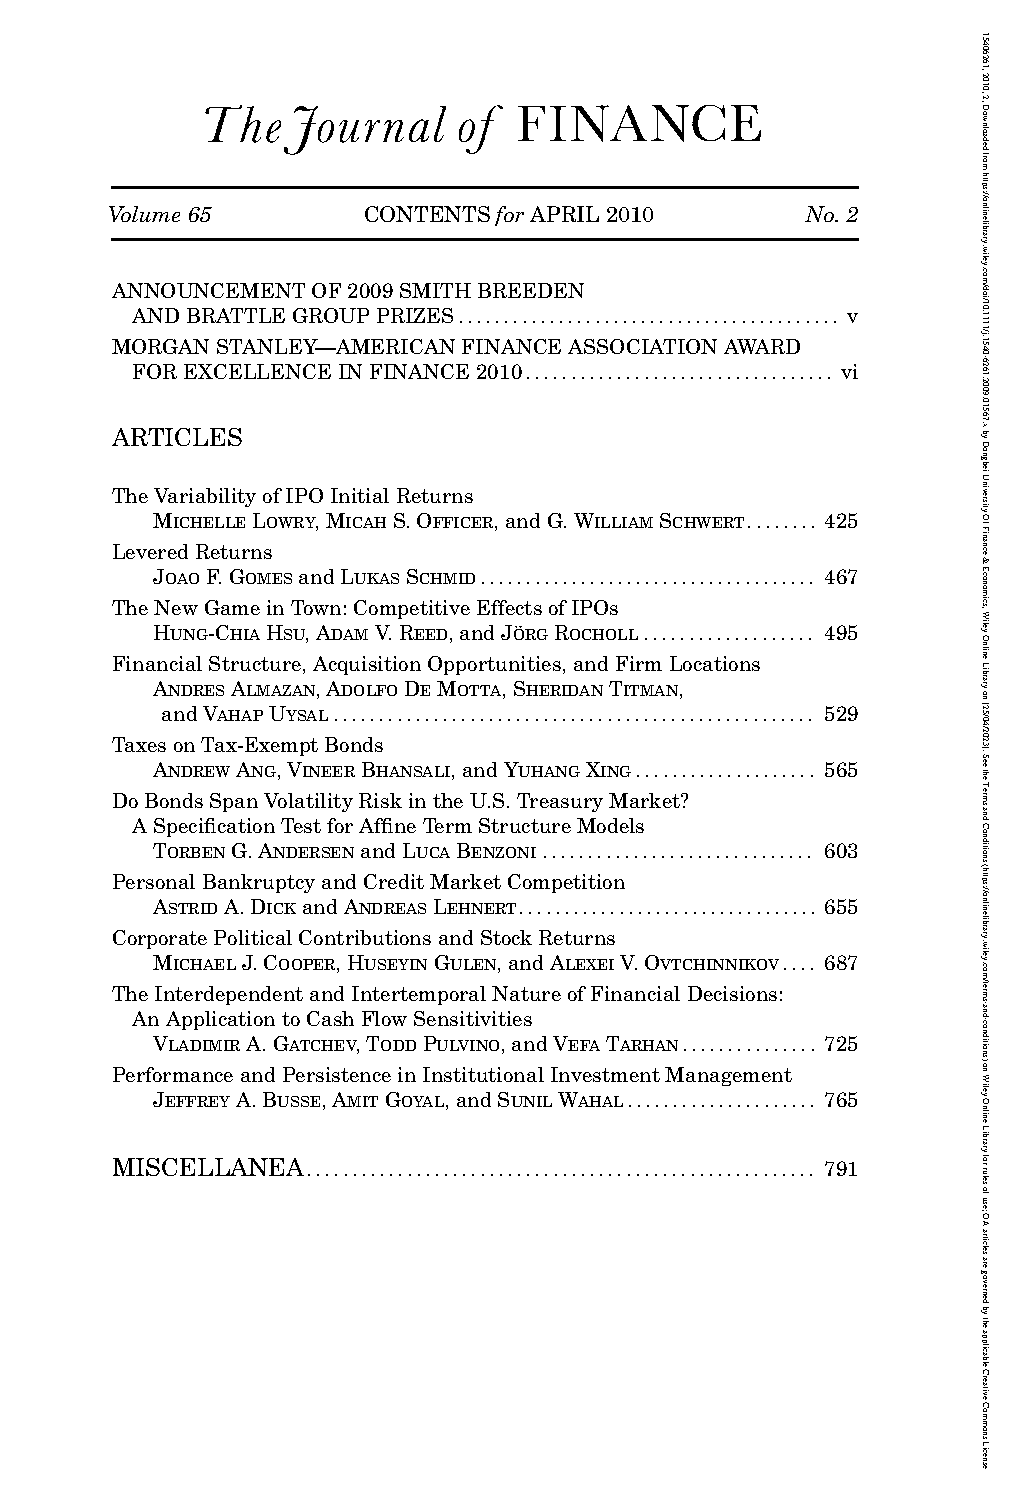
\includegraphics[width=0.6\linewidth]{Files/Front}
	\end{figure}

\end{frame}

\begin{frame}{Q-factor}
	\begin{itemize}
		\item \begin{figure}
			\centering
			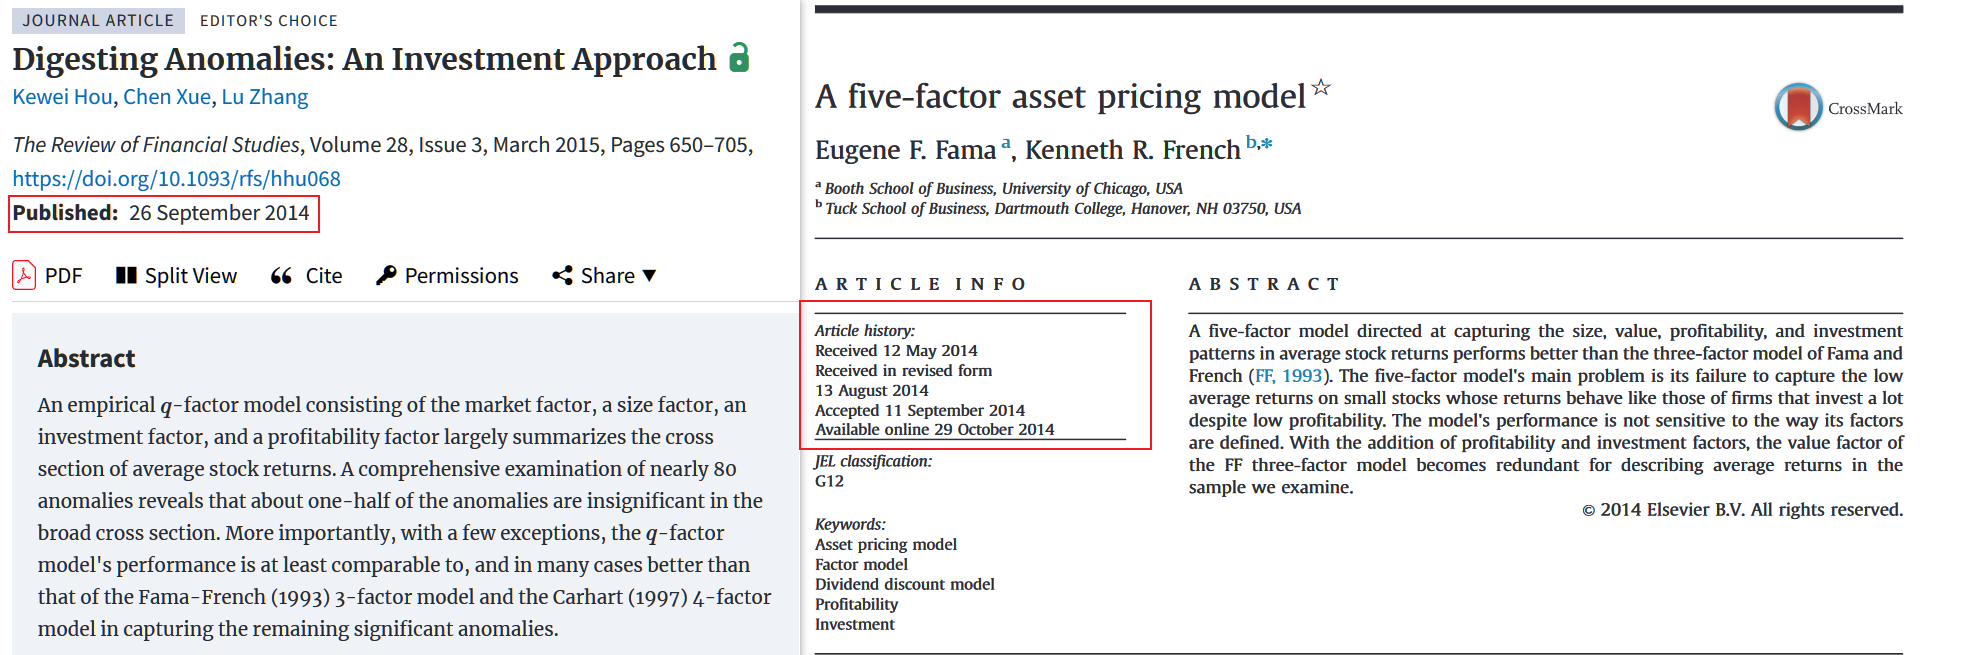
\includegraphics[width=1.1\linewidth]{Files/pk.png}
		\end{figure}
	\end{itemize}
\end{frame}


\end{document} 